\section{MEASURED HVAC EVIDENCE AND SENSITIVITY}
\noindent The primary measured application uses the collection of \cite{granderson2020data}, specifically Figshare article 11752740, version 3, under its CC0 dedication. Only SZCAV.csv and SZVAV.csv are selected. Source checksums, inventory tables, all day assignments, public summaries and selected one-minute signals are saved with the evidence. The original CSV downloads remain outside Git. The source contains manually imposed faults on one FLEXLAB air handler; labels are experimentally established conditions, while scheduling and weighted consequences are constructed.\draftcredit

\subsection{Source and Information Boundaries}
All 26 recorded days are included, with eight development days and 18 evaluation days. Each contributes three windows, totaling 78 distinct source windows. The initial and revised development collections reuse the same 24 development windows and do not create additional source units. Evaluation has one generation replicate. Source date, filename, fault indicator and imposed-condition description are evaluator-only. Control mode and recording hour are public. Dates are not needed for diagnosis and are excluded to reduce answer-bearing metadata exposure. Public-source pretraining contamination cannot be ruled out.

The three tickets from an experimental day are correlated snapshots of the same equipment under the same imposed condition. They are retrospectively available after the final window closes. Their simultaneous arrival is an assumed backlog condition, not an observed pattern of building fault incidence. A policy changes a recorded diagnosis, not a sensor trajectory. Labels support diagnosis scoring but cannot establish repair efficacy, energy savings or physical harm prevention.

Ten channels retain original Fahrenheit units and fractional controls. Means, minima, maxima and first-to-last changes are deterministic within-window summaries. No evaluation normalization is fit. The conventional classifier standardizes 42 public features, comprising 40 statistics, mode and hour, using development means and standard deviations. Zero-variance dimensions receive scale one. It assigns the closest class centroid by squared Euclidean distance. It is a transparent baseline rather than a tuned state-of-the-art fault detector.

\begin{table*}[t]
\caption{Measured-data evaluation by experimentally annotated component category. Counts are windows, nested within experimental days on one unit. Proposed and reviewed labels are generated. The conventional baseline uses development data only.}
\centering\small
\begin{tabular}{lrrrrr}
\toprule
Condition & Days & Windows & Proposal correct & Review correct & Baseline correct \\
\midrule
normal & 3 & 9 & 1 & 1 & 6 \\
outdoor damper & 4 & 12 & 0 & 0 & 7 \\
heating valve & 6 & 18 & 18 & 12 & 14 \\
cooling valve & 5 & 15 & 0 & 1 & 0 \\
\bottomrule
\end{tabular}
\end{table*}


\subsection{Frozen Conditions and Resource Use}
The declaration fixes six policies, two weight schemes, one or two review slots, service times one/two/three, and three review-benefit conditions. These give 216 paired policy runs per experimental day and 3,888 total. The primary signed-gain rule, secondary risk-only ablation and ideal reference all reuse the same generated proposal/review pair for each window. No policy gets privileged observations. Review output takes effect only at completed service; invalid output preserves the proposal, while abstention is unresolved. Reviews must finish by cutoff equality. No late result cancels an incurred loss.

Development uses 48 initial and 48 revised calls. Evaluation adds 108 calls. All 204 GPU attempts succeed, with no retry, using 125,765 prompt tokens and 9,131 completion tokens. Maximum actual input and output lengths are 745 and 93 tokens, within the existing 2,048-token context and 128-token output allowance. Total measured generation-request time is 174.66 seconds, and the slowest attempt is 1.73 seconds. This measured latency is distinct from assumed review service time. GPU evidence verifies BF16 on the RTX 6000 Ada, the pinned Qwen revision and zero CPU offloading. Server token and call deltas reconcile exactly.

Signed-gain admission declines all primary reviews because fitted gains are nonpositive. That rule misses the one realized potentially helpful model review while avoiding six harmful changes. These are consequences of a sparse development fit, not an oracle identifying harmful evaluation cases. Review-pair diagnostics contain five wrong-category introductions and one harmful abstention. Four further abstentions occur on already wrong proposals. Aggregate error-risk AUROC is 0.5023, Brier score 0.2305, pooled-development Brier 0.2349 and constant-half Brier 0.2500. The prediction ranking is nearly uninformative despite its modest Brier improvement over the constant reference.

\begin{figure*}[t]
\centering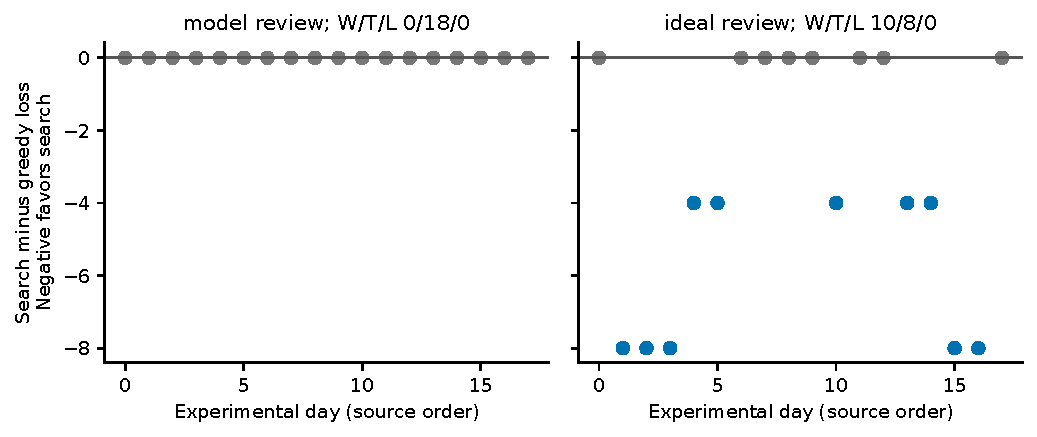
\includegraphics[width=0.98\textwidth]{../artifacts/stage7_empirical/figures/paired_differences.pdf}
\caption{All 18 experimental-day search-minus-greedy differences. Outcomes combine generated diagnoses with annotated correctness and simulated deadlines and weights. The left panel's zero differences follow from a shared admission rule that declines model review. The ideal reference on the right uses corrected labels only at review completion. Days share one physical unit and are not independent buildings.}
\end{figure*}

\begin{figure*}[t]
\centering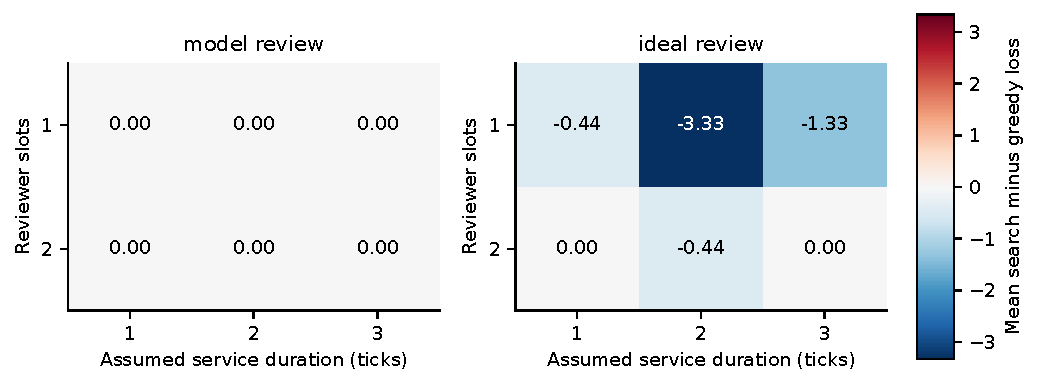
\includegraphics[width=0.98\textwidth]{../artifacts/stage7_empirical/figures/capacity_sensitivity.pdf}
\caption{Prespecified simulated capacity and duration sensitivity on saved measured-data proposals. Cell values are mean search-minus-greedy weighted diagnosis loss. The color scale is centered at zero. Signed model-review admission produces mechanical ties. Ideal review exposes a conditional ordering benefit. These abstract capacities and time units are not measurements of human inspection.}
\end{figure*}

\begin{figure*}[t]
\centering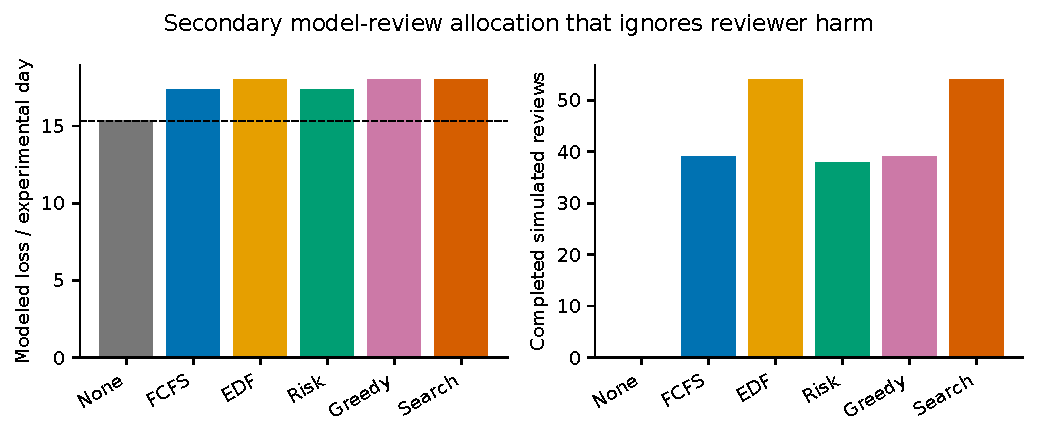
\includegraphics[width=0.98\textwidth]{../artifacts/stage7_empirical/figures/risk_only_secondary.pdf}
\caption{Secondary allocation that substitutes error probability for reviewer effectiveness. The same saved model responses are applied. Loss and review counts are simulated, while correctness is determined by experimental labels. More reviews do not improve diagnosis. Search and greedy tie despite different sequences on 15 of 18 days. The dashed line is no-review loss.}
\end{figure*}

\begin{figure*}[t]
\centering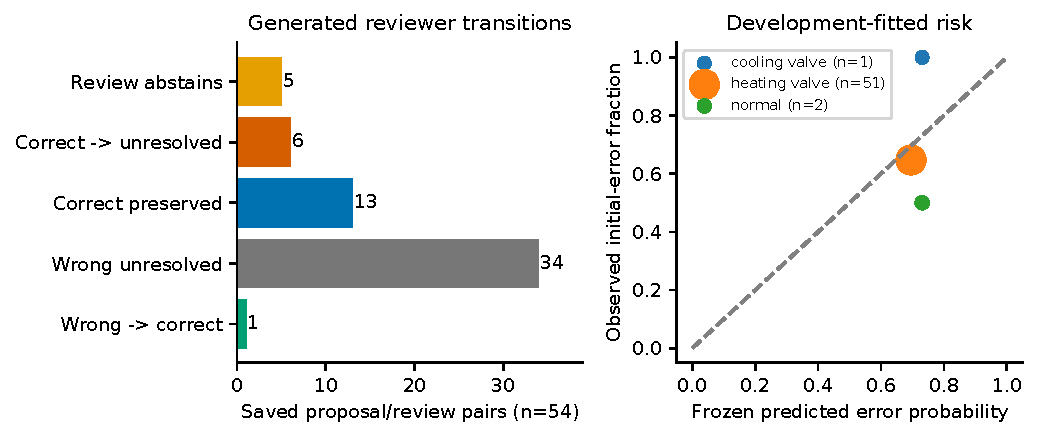
\includegraphics[width=0.98\textwidth]{../artifacts/stage7_empirical/figures/reviewer_risk.pdf}
\caption{Generated reviewer transitions and development-fitted risk on 54 evaluation windows. One correct-to-unresolved transition is an abstention; five change to wrong categories. Abstentions overlap the transition categories. The calibration plot identifies counts for each proposed category, with highly tied risks and small bins. Ground-truth labels are used only in this offline diagnosis, not at dispatch.}
\end{figure*}

\subsection{First-Qualifying Queue Examples}
The rule selects the first numerical source run satisfying each comparison sign, without ranking by effect magnitude. The primary model-review condition has only ties. Its first tie is run01, where no reviews are admitted. The ideal reference has a first benefit at run02, with difference $-8$, and a first tie at run01. Neither has an unfavorable search-minus-greedy case under the declared primary capacity. Absence is reported rather than replacing the rule with a favorable example from another configuration.

\begin{figure*}[t]
\centering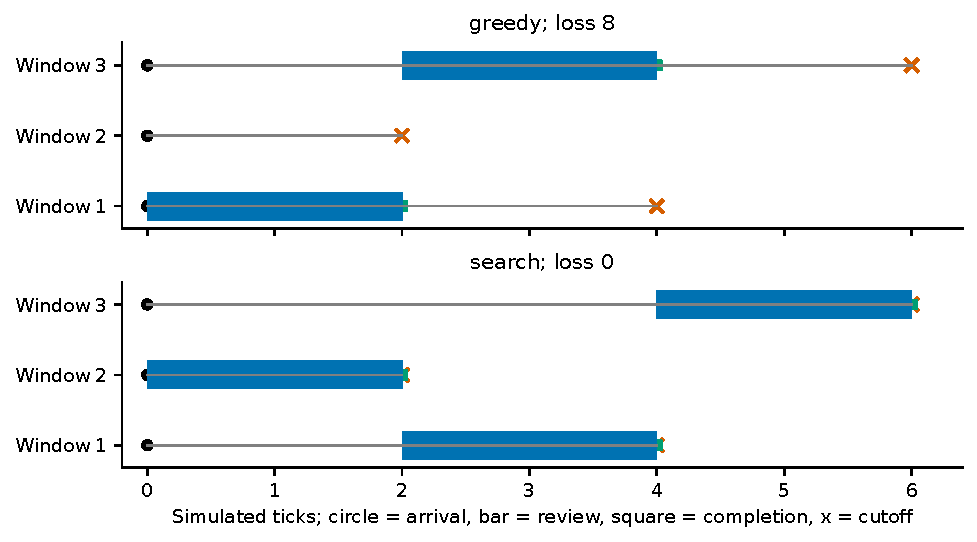
\includegraphics[width=0.88\textwidth]{../artifacts/stage7_empirical/figures/queue_ideal_benefit.pdf}
\caption{First ideal-reference benefit, run02. Both policies receive the same generated diagnoses from measured sensor windows. Bars show simulated review occupancy, squares completion and crosses cutoffs. Search preserves a timely review that greedy misses. Ideal correction is an assumption and this figure is not evidence of successful physical repair.}
\end{figure*}

\begin{figure*}[t]
\centering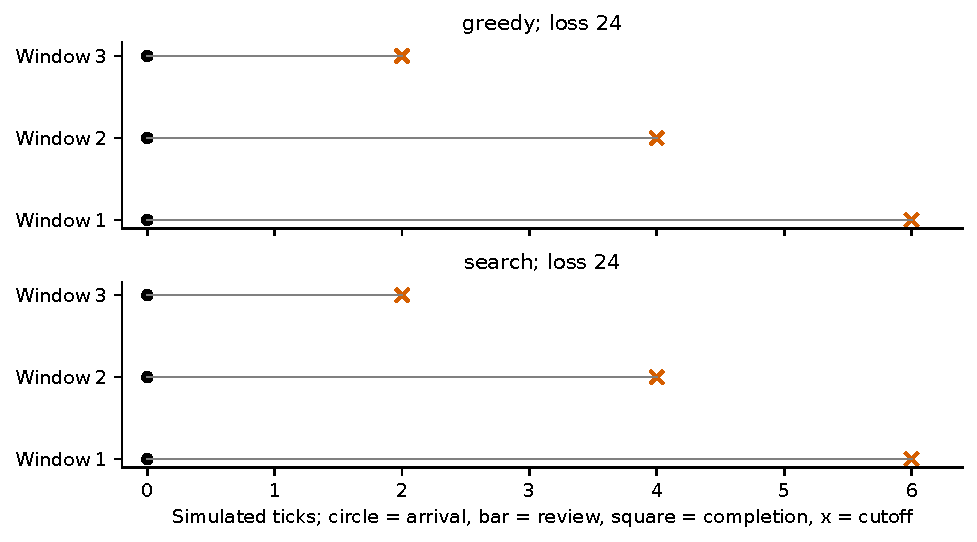
\includegraphics[width=0.88\textwidth]{../artifacts/stage7_empirical/figures/queue_model_tie.pdf}
\caption{First primary-condition tie, run01. All three diagnosis tickets arrive together, but the development-fitted signed gain admits no model reviews. The displayed cutoff events are simulated. Empty review bars reflect the declared decision rule, not missing execution records.}
\end{figure*}

\subsection{Secondary Application Access and Reproduction}
BIRD-Critic-SQLite public records omit reference solutions and hidden tests; the official repository offers them through email contact. No contact was made. BIRD-SQL provides accessible development references and database downloads, but its required database audit and execution study did not fit the remaining original execution deadline. No SQL or optional synthetic fraud result is claimed. This keeps a completed measured primary study separate from unexecuted applications.

The saved-output command is \texttt{bash scripts/replay\_stage7.sh}. It verifies every attempt, frozen input, source summary and policy trace, recomputes tables in a temporary directory, regenerates vector figures, and builds the manuscript and supplement. It does not change the frozen traces or their measured planning latency. Exact GPU regeneration uses the recorded public task files and role prompts, but requires a new explicit authorization and fresh output directory after the historical deadline. Seed reuse alone does not guarantee identical generations.
